%%----------------------------------------------------------------------------
%% Presentatie HoGent Bedrijf en Organisatie
%%----------------------------------------------------------------------------
%% Auteur: Bert Van Vreckem [bert.vanvreckem@hogent.be]

\documentclass{beamer}

%==============================================================================
% Aanloop
%==============================================================================

%---------- Packages ----------------------------------------------------------
\usepackage{etex}
\usepackage{graphicx,multicol}
\usepackage{comment,enumerate,hyperref}
\usepackage{amsmath,amsfonts,amssymb}
\usepackage{tikz}
\usepackage[dutch]{babel}
\usepackage[utf8]{inputenc}
\usepackage{multirow}
\usepackage{eurosym}
\usepackage{listings}
\usepackage[T1]{fontenc}
\usepackage{lmodern}
\usepackage{textcomp}
\usepackage{framed}
\usepackage{wrapfig}
\usepackage{pgf-pie}
\usepackage{pgfplots}
\usepackage{booktabs}
\usepackage{pgfplotstable}
\usepackage{changepage}

%---------- Configuratie ------------------------------------------------------

\usetikzlibrary{arrows,shapes,backgrounds,positioning,shadows}
\usetikzlibrary{pgfplots.statistics}


\lstset{ %
  language=R,                     % the language of the code
  float=H,
  basicstyle=\tiny,       % the size of the fonts that are used for the code
  numbers=left,                   % where to put the line-numbers
  numberstyle=\tiny\color{HoGentGrey},  % the style that is used for the line-numbers
  stepnumber=1,                   % the step between two line-numbers. If it's 1, each line
  % will be numbered																
  numbersep=5pt,                  % how far the line-numbers are from the code
  backgroundcolor=\color{white},  % choose the background color. You must add \usepackage{color}
  showspaces=false,               % show spaces adding particular underscores
  showstringspaces=false,         % underline spaces within strings
  showtabs=false,                 % show tabs within strings adding particular underscores
  frame=single,                   % adds a frame around the code
  rulecolor=\color{black},        % if not set, the frame-color may be changed on line-breaks within not-black text (e.g. commens (green here))
  tabsize=2,                      % sets default tabsize to 2 spaces
  captionpos=b,                   % sets the caption-position to bottom
  breaklines=true,                % sets automatic line breaking
  breakatwhitespace=false,        % sets if automatic breaks should only happen at whitespace
  title=\lstname,                 % show the filename of files included with \lstinputlisting;
  % also try caption instead of title
  keywordstyle=\color{HoGentBlue}, % keyword style
  commentstyle=\color{HoGentGrey}, % comment style
  stringstyle=\color{HoGentRed},  % string literal style
  escapeinside={\%*}{*)},         % if you want to add a comment within your code
  morekeywords={*,...}            % if you want to add more keywords to the set
} 

\usetheme{hogent}
\setbeameroption{show notes}

%---------- Commando-definities -----------------------------------------------

\newcommand{\tabitem}{~~\llap{\textbullet}~~}
\renewcommand{\arraystretch}{1.2}

%---------- Info over de presentatie ------------------------------------------

\title[Intro]{Onderzoekstechnieken\\Les 3. Steekproefonderzoek}
\author{Jens Buysse \and Wim {De Bruyn} \and Wim Goedertier \and Bert {Van Vreckem}}
\date{AJ 2017-2018}

%==============================================================================
% Inhoud presentatie
%==============================================================================

\begin{document}

%---------- Front matter ------------------------------------------------------

% Dia met het HoGent logo
\HoGentLogo

% Titeldia met faculteitslogo
\titleframe

%---------- Inhoud ------------------------------------------------------------

\begin{frame}
  \frametitle{What's on the menu today?}

  \tableofcontents
\end{frame}

\section{Steekproefonderzoek}
\sectionframelogo{USA Today has come out with a new survey. Apparently, three out of every four people make up 75\% of the population\\

  --David Letterman
}

\begin{frame}
  \frametitle{Steekproef en Populatie}
  Herinner onze superhelden
  \begin{tikzpicture}[xscale=4,yscale=2]
    \draw (0,2) -- (0,0);
    \foreach \num/\label in {0/0, 0.2/20, .4/40, .6/60, .8/80, 1/100, 1.2/120, 1.4/140, 1.6/160, 1.8/180, 2/200}{%
      \draw (0, \num) -- (2.5, \num);
      \draw[shift={(0, \num)}] (1pt,0pt) -- (-1pt,0pt) node[left] {\scriptsize \label};
    }

    \node[anchor=north] (hero1) at (0.3,1.5)
    {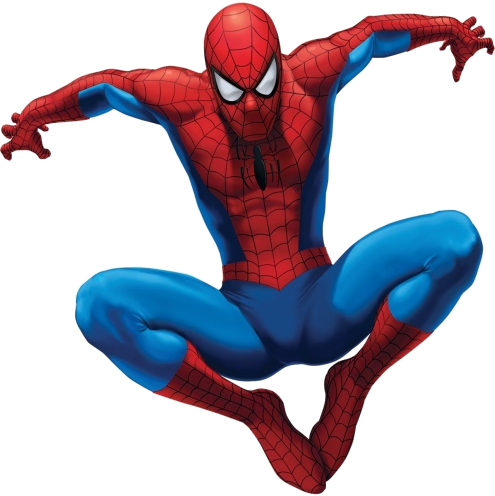
\includegraphics[height=2.9cm]{img/les2-hero-1}};
    \node[anchor=north] (hero2) at (0.8,2.05)
    {
\includegraphics[height=4cm]{img/les2-hero-2}};
    \node[anchor=north] (hero3) at (1.3,1.575)
    {
\includegraphics[height=3.1cm]{img/les2-hero-3}};
    \node[anchor=north] (hero4) at (1.8,2.1)
    {
\includegraphics[height=4.1cm]{img/les2-hero-4}};
    \node[anchor=north] (hero5) at (2.3,1.95)
    {
\includegraphics[height=3.8cm]{img/les2-hero-5}};

    \node (size1) at (0.3, 1.5) {\scriptsize 141 cm};
    \node (size2) at (0.8, 2.1) {\scriptsize 198 cm};
    \node (size3) at (1.3, 1.51) {\scriptsize 143 cm};
    \node (size4) at (1.8, 2.15) {\scriptsize 201 cm};
    \node (size5) at (2.3, 1.95) {\scriptsize 184 cm};
  \end{tikzpicture}
\end{frame}

\begin{frame}
  \frametitle{Steekproef en Populatie}

  \begin{figure}
    \centering
    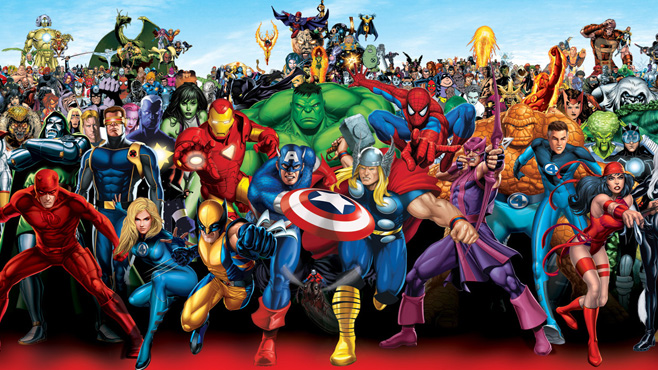
\includegraphics[width=1.00\textwidth]{img/les5-heroes.jpg}
    \label{fig:les5-heroes}
  \end{figure}

\end{frame}

\begin{frame}
  \frametitle{Steekproef en Populatie}
  \brightbox{ De verzameling van alle objecten of personen waar men in geïnteresseerd is voor het onderzoek noemt men de \textcolor{HoGentAccent6}{populatie}.}

  \brightbox{ Wanneer men een subgroep uit een populatie gaat onderzoeken, dan noemen we die groep een \textcolor{HoGentAccent6}{steekproef}.}

  \begin{center}
    \begin{tikzpicture}
      \fill[HoGentAccent4] (2,2) ellipse (4cm and 2 cm) ;
      \fill[HoGentAccent2] (2,2) ellipse (2cm and 1cm) ;
      \node[draw=none,minimum size=1cm,inner sep=0pt] at (3,0.5) {populatie};
      \node[draw=none,minimum size=1cm,inner sep=0pt] at (3,2) {steekproef};
    \end{tikzpicture}
  \end{center}
\end{frame}

\begin{frame}
  \frametitle{Methode om tot een steekproef te komen}
  \begin{center}
    \begin{tikzpicture}[
        auto, thick, ->, >=stealth', shorten >=1pt, node distance=2cm,
        fase/.style={ shape=rectangle, fill=HoGentFBO, text=white, draw}
      ]

    \node[fase] (1) { Definitie van populatie };
    \node[fase] (2) [below of=1] { Bepalen van steekproefkader };
    \node[fase] (3) [below of=2] { Budget en tijd };

    \draw (1) -- (2);
    \draw (2) -- (3);
    \end{tikzpicture}
  \end{center}

\end{frame}

\begin{frame}
  \frametitle{Gestratificeerd naar variabelen}

  \begin{center}
    \begin{tabular}{l|cccc|c}
      & \multicolumn{4}{c|}{\textbf{Leeftijd}} & \\
      Geslacht & $\le 18$ & $]18,25]$ & $]25, 40]$ & $> 40$ & Totaal\\
      \hline
      Vrouw & 500 & 1500 & 1000 & 250 & 3250 \\
      Man   & 400 & 1200 & 800 & 160 & 2560\\
      \hline
      Totaal & 900 & 2700 & 1800 & 410 & 5810
    \end{tabular}

    \vspace{1cm}

    \pause
    \begin{tabular}{l|cccc|c}
      & \multicolumn{4}{c|}{\textbf{Leeftijd}} & \\
      Geslacht & $\le 18$ & $]18,25]$ & $]25, 40]$ & $> 40$ & Totaal\\
      \hline
      Vrouw & 50 & 150 & 100 & 25 & 325 \\
      Man   & 40 & 120 & 80 & 16 & 256\\
      \hline
      Totaal & 90 & 270 & 180 & 41 & 581
    \end{tabular}

  \end{center}
\end{frame}

\begin{frame}
  \frametitle{Hoe elementen voor een steekproef kiezen?}

  \begin{description}
    \item[Aselecte steekproef] elk element uit de onderzoekspopulatie heeft een even grote kans om in de steekproef terecht te komen
    \item[Selecte steekproef] of een element in de steekproef terecht komt is afhankelijk van een persoonlijke beoordeling van een onderzoeker
  \end{description}

  \begin{center}
    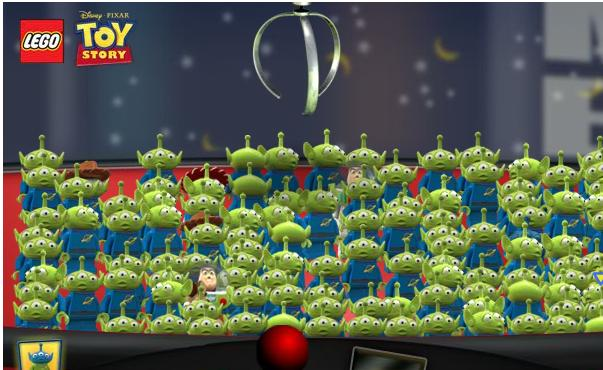
\includegraphics[width=.5\textwidth]{img/les4-aselect}
  \end{center}
\end{frame}

\begin{frame}
  \frametitle{Mogelijke fouten}

  \begin{itemize}
    \item<+-> Toevallige steekproeffouten
      \begin{itemize}
        \item Puur toeval
      \end{itemize}
    \item<+-> Systematische steekproeffouten
      \begin{itemize}
        \item bv. online enquête: wat met deel van de populatie die geen computer heeft?
      \end{itemize}
    \item<+-> Toevallige niet-steekproeffouten
      \begin{itemize}
        \item Verkeerd aangekruiste antwoorden
      \end{itemize}
    \item<+-> Systematische niet-steekproeffouten
      \begin{itemize}
        \item Respondenten met sterke band met onderwerp van onderzoek reageren positief terwijl anderen niet reageren
      \end{itemize}
  \end{itemize}
\end{frame}

\begin{frame}
  \frametitle{Variantie/standaarddeviatie van een steekproef}

  \begin{center}
    Aangepaste formule:
    
    \begin{equation*}
    s^2 = \frac{1}{\alert{n-1}} \sum_{i=1}^{n} (\overline{x} - x_i)^2
    \end{equation*}
    
    De reden voor de wijziging kan je wiskundig bewijzen, maar we gaan het empirisch onderzoeken

    \vfill

    Java applet: \url{http://www.uvm.edu/~dhowell/SeeingStatisticsApplets/N-1.html}
    \vfill
    R-script: \href{https://github.com/HoGentTIN/onderzoekstechnieken-cursus/blob/master/cursus/data/sample-variance.R}{cursus/data/sample-variance.R}
  \end{center}
\end{frame}

\section{Kansverdeling van een steekproef}

\begin{frame}
  \frametitle{Wat weten we nog van de kansrekening?}

  \begin{itemize}
    \item Uitkomstenruimte
    \item Uitkomst
    \item Gebeurtenis
    \item Kansruimte
  \end{itemize}

  \vfill

  \hfill 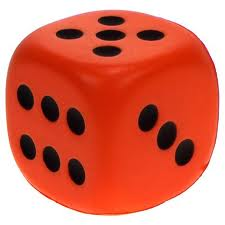
\includegraphics[width=.2\textwidth]{img/les04-dobbelsteen}
\end{frame}

\begin{frame}
  \frametitle{Kansverdeling voor één dobbelsteen}

  Wat is de kans om een aantal ogen te werpen met een dobbelsteen?

  \begin{center}
    \begin{tabular}{|c|c|c|c|c|c|}
      \hline
      1&2&3&4&5&6\\
      \hline
      \onslide<2->{$\frac{1}{6}}$ &\onslide<2->{$\frac{1}{6}}$ &\onslide<2->{$\frac{1}{6}}$ &\onslide<2->{$\frac{1}{6}}$ &\onslide<2->{$\frac{1}{6}}$ &     \onslide<2->{$\frac{1}{6}}$ \\
      \hline

    \end{tabular}
  \end{center}

  \onslide<2->{%
  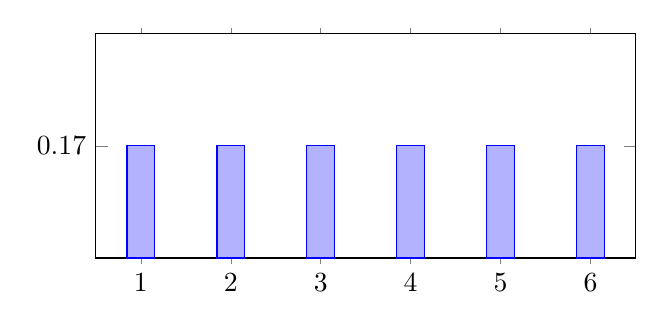
\begin{tikzpicture}
    \begin{axis}[ybar,ytick=data, anchor=north, yscale=.5]
      \addplot
      coordinates {
        (1, 1/6)
        (2, 1/6)
        (3, 1/6)
        (4, 1/6)
        (5, 1/6)
        (6, 1/6)};
    \end{axis}
  \end{tikzpicture}}
\end{frame}

\begin{frame}
  \frametitle{Kansverdeling voor twee dobbelstenen}

  \begin{center}
    \begin{tabular}{|c|c|c|c|c|c|c|c|c|c|c|c|}
      \hline
      2&3&4&5&6&7&8&9&10&11&12\\
      \hline
      \onslide<2->{$\frac{1}{36}}$ &\onslide<2->{$\frac{2}{36}}$ &\onslide<2->{$\frac{3}{36}}$ &\onslide<2->{$\frac{4}{36}}$ &\onslide<2->{$\frac{5}{36}}$ & \onslide<2->{$\frac{6}{36}}$ & \onslide<2->{$\frac{5}{36}}$ &\onslide<2->{$\frac{4}{36}}$ & \onslide<2->{$\frac{3}{36}}$ &\onslide<2->{$\frac{2}{36}}$ &\onslide<2->{$\frac{1}{36}}$ \\
      \hline

    \end{tabular}
  \end{center}

  \onslide<2->{%
  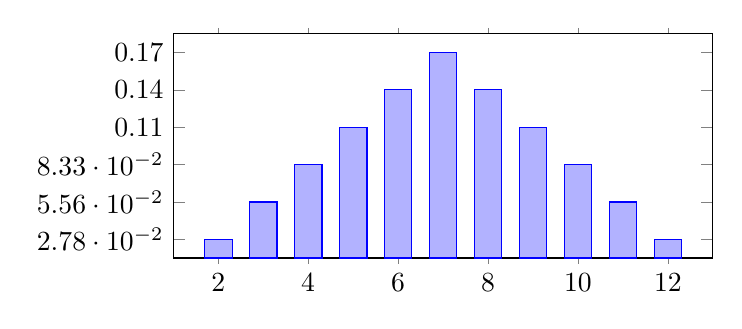
\begin{tikzpicture}
    \begin{axis}[ybar,ytick=data, anchor=north, yscale=.5]
      \addplot
      coordinates {
        (2, 1/36)
        (3, 2/36)
        (4, 3/36)
        (5, 4/36)
        (6, 5/36)
        (7, 6/36)
        (8, 5/36)
        (9, 4/36)
        (10, 3/36)
        (11, 2/36)
        (12, 1/36)
      };

    \end{axis}
  \end{tikzpicture}}

\end{frame}

  \pgfmathdeclarefunction{gauss}{2}{%
    \pgfmathparse{1/(#2*sqrt(2*pi))*exp(-((x-#1)^2)/(2*#2^2))}%
  }

\begin{frame}
  \frametitle{Continue kansverdeling}

  De reactiesnelheid van Superman kan als volgt weergegeven worden:

  \vspace{1cm}

  \begin{tikzpicture}
\begin{axis}[
  domain=0:10, samples=100,
  axis lines*=left, xlabel=$x$, ylabel=$y$,
  every axis y label/.style={at=(current axis.above origin),anchor=south},
  every axis x label/.style={at=(current axis.right of origin),anchor=west},
  height=5cm, width=12cm,
  xtick={5,3.5,6.5}, ytick=\empty,
  enlargelimits=false, clip=false, axis on top,
  grid = major
  ]
  \addplot [fill=cyan!20, draw=none, domain=0:9] {gauss(5,1.5)} \closedcycle;
  \draw [yshift=-0.6cm, latex-latex](axis cs:3.5,0) -- node [fill=white] {$\sigma$} (axis cs:5.0,0);
  \end{axis}
  \end{tikzpicture}
  \hfill
\includegraphics[width=1.5cm]{img/les2-hero-3}
\end{frame}

\begin{frame}
  \frametitle{Standaardnormale verdeling}

  % Bron: http://johncanning.net/wp/?p=1202
  \begin{center}
    \begin{tikzpicture}
      \begin{axis}[
          no markers, domain=0:10, samples=100,
          axis lines*=left,height=6cm, width=10cm,
          xtick={-3, -2, -1, 0, 1, 2, 3}, ytick=\empty,
          enlargelimits=false, clip=false, axis on top,
          grid = major
        ]
        \addplot [smooth,fill=cyan!20, draw=none, domain=-3:3] {gauss(0,1)} \closedcycle;
        \addplot [smooth,fill=orange!20, draw=none, domain=-3:-2] {gauss(0,1)} \closedcycle;
        \addplot [smooth,fill=orange!20, draw=none, domain=2:3] {gauss(0,1)} \closedcycle;
        \addplot [smooth,fill=blue!20, draw=none, domain=-2:-1] {gauss(0,1)} \closedcycle;
        \addplot [smooth,fill=blue!20, draw=none, domain=1:2] {gauss(0,1)} \closedcycle;
        \addplot[<->] coordinates {(-1,0.4) (1,0.4)};
        \addplot[<->] coordinates {(-2,0.3) (2,0.3)};
        \addplot[<->] coordinates {(-3,0.2) (3,0.2)};
        \node[coordinate, pin={68.3\%}] at (axis cs: 0, 0.35){};
        \node[coordinate, pin={95.4\%}] at (axis cs: 0, 0.25){};
        \node[coordinate, pin={99.7\%}] at (axis cs: 0, 0.15){};
        \node[coordinate, pin={34.1\%}] at (axis cs: -0.5, 0){};
        \node[coordinate, pin={34.1\%}] at (axis cs: 0.5, 0){};
        \node[coordinate, pin={13.6\%}] at (axis cs: 1.5, 0){};
        \node[coordinate, pin={13.6\%}] at (axis cs: -1.5, 0){};
        \node[coordinate, pin={2.1\%}] at (axis cs: 2.5, 0){};
        \node[coordinate, pin={2.1\%}] at (axis cs: -2.5, 0){};
      \end{axis}
    \end{tikzpicture}
  \end{center}
\end{frame}

\begin{frame}
  \frametitle{Hoe groot is de kans dat\dots}

  Zijn reactiesnelheid langer is dan 6,5 milliseconden?
  
  Wisk. notatie: $P( x > 6,5)$

  \vspace{2cm}

  \begin{itemize}
    \item $z$-tabel (of R-functie \texttt{pnorm})
    \item Symmetrieregel
    \item Regel van 100\% kans
  \end{itemize}
\end{frame}

\begin{frame}
  \frametitle{De $z$-score}
  
  \begin{itemize}
    \item Stel, $x \in X \sim Nor(\mu, \sigma)$
    \item Welke $z \in Z \sim Nor(0, 1)$ ligt op dezelfde positie van de Gauss-curve?
    \pause
    \item Antwoord: $z = \frac{x - \mu}{\sigma}$
  \end{itemize}
  
\end{frame}

\begin{frame}[fragile]
  \frametitle{Belangrijkste functies in R}
  
  Voor een normale verdeling met gemiddelde \texttt{m} en standaardafwijking \texttt{s}:
  \vfill
  \centering
  \begin{tabular}{ll}
  	\textbf{Functie}      & \textbf{Betekenis}                          \\ \hline
  	\verb|pnorm(x, m, s)| & Linkerstaartkans, $P(X<\mathtt{x})$         \\
  	\verb|dnorm(x, m, s)| & Hoogte van de Gausscurve op punt \texttt{x} \\
  	\verb|qnorm(p, m, s)| & Onder welke grens zal \texttt{p}\% van de   \\
  	                      & waarnemingen liggen?                        \\
  	\verb|rnorm(n, m, s)| & Genereer \texttt{n} normaal verdeelde random getallen
  \end{tabular}
  \vfill
  Argumenten \texttt{m} en \texttt{s} weglaten geeft waarden voor de standaardnormaalverdeling.
\end{frame}

\begin{frame}
  \frametitle{Berekeningswijzen}

  \begin{enumerate}
    \item Hoe groot is de kans dat de reactiesnelheid van Superman minder dan 4 ms is?
    \item Hoe groot is de kans dat hij in minder dan 7 ms reageert?
    \item Hoe groot is de kans dat Superman in minder dan 3 ms reageert?
    \item Hoe groot is de kans dat hij reageert tussen de 2 en de 6,5 ms?
    \item Binnen welke tijd ligt 80\% van zijn reactiesnelheid?
  \end{enumerate}
\end{frame}

\begin{frame}
  \frametitle{Vraag 3: $P(X<3)$}

  \begin{tikzpicture}
  \begin{axis}[no markers,domain=-4:4,axis lines*=left,yscale=.7,enlargelimits=false,clip=false]
    \addplot[very thick,smooth,draw=HoGentFBO]{gauss(0, 1)};
    \addplot[smooth,fill=black!20, draw=black, domain=-4:-4/3] {gauss(0,1)} \closedcycle;

    \node at (axis cs: -1.33, -.05) {\small -1.33};
  \end{axis}
  \end{tikzpicture}
\end{frame}

\begin{frame}
  \frametitle{Vraag 4: $P(2<X<6,5)$}

  \begin{tikzpicture}
  \begin{axis}[no markers,domain=-4:4,axis lines*=left,yscale=.7,enlargelimits=false,clip=false]
    \addplot[very thick,smooth,draw=HoGentFBO]{gauss(0, 1)};
    \addplot[smooth,fill=black!20, draw=black, domain=-2:1] {gauss(0,1)} \closedcycle;

    \node at (axis cs: 1, -.05) {\small 1};
  \end{axis}
  \end{tikzpicture}
\end{frame}

\begin{frame}
  \frametitle{Vraag 5}

  Voor welke $x$ is $P(X<x) = 80\%$?

  \vfill

  \begin{tikzpicture}
  \begin{axis}[no markers,domain=-4:4,axis lines*=left,yscale=.7,enlargelimits=false,clip=false]
    \addplot[very thick,smooth,draw=HoGentFBO]{gauss(0, 1)};
    \addplot[smooth,fill=black!20, draw=black, domain=-4:.84] {gauss(0,1)} \closedcycle;

    \node at (axis cs: .84, -.05) {\small .84};
  \end{axis}
  \end{tikzpicture}
\end{frame}

\section{De Centrale Limietstelling}
\sectionframelogo{}


\begin{frame}
  \frametitle{De centrale limietstelling}

  \brightbox{Als de steekproefomvang voldoende groot is, dan kan de kansverdeling van het steekproefgemiddelde benaderd worden met een normale verdeling. Dit geldt ongeacht de vorm van de kansverdeling van de individuele waarnemingen}

  \vfill

  \begin{columns}[c]
    \column{.33\textwidth}
    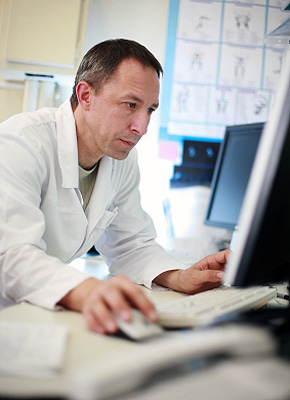
\includegraphics[width=2cm]{img/les4-centrlimiet}
    \column{.33\textwidth}
    \begin{itemize}
      \item 1 test
      \item 25 tests
      \item 100 tests
    \end{itemize}
    \column{.33\textwidth}
    
\includegraphics[width=2cm]{img/les2-hero-3}
  \end{columns}

Demo: \url{https://students.brown.edu/seeing-theory/probability-distributions/index.html}

\end{frame}

\begin{frame}
  \frametitle{De centrale limietstelling}
  Beschouw een aselecte steekproef van $n$ waarnemingen die uit een willekeurige populatie met verwachting $\mu$ en standaardafwijking $\sigma$ wordt genomen. Als $n$ groot genoeg is zal de kansverdeling van $\overline{x}$ een normale verdeling benaderen met verwachting $\mu_{\overline{x}} = \mu$ en standaardafwijking $\sigma_{\overline{x}} = \frac{\sigma}{\sqrt{n}}$. Hoe groter de steekproef is, des te beter zal de normale benadering van de kansverdeling van $\overline{x}$ zijn.
\end{frame}

\section{Van steekproef naar populatie}
\sectionframelogo{}

\begin{frame}
  \frametitle{Puntschatter}
    \brightbox{Een puntschatter voor een populatieparameter is een regel of een formule die ons zegt hoe we uit de steekproef een getal moeten berekenen om de populatieparameter te schatten.}
\end{frame}

\subsection{Betrouwbaarheidsintervallen}
\begin{frame}
  \frametitle{Betrouwbaarheidsinterval}
  \brightbox{Een \textcolor{HoGentAccent6}{betrouwbaarheidsinterval} is een regel of een formule die ons zegt hoe we uit de steekproef een interval kunnen berekenen dat de waarde van de parameter met een zeker \textcolor{HoGentAccent6}{betrouwbaarheidsniveau} bevat.}
\end{frame}

\subsection{Betrouwbaarheidsinterval grote steekproef}


\begin{frame}
\frametitle{Betrouwbaarheidsinterval}

Gegeven een steekproef met gemiddelde $\overline{x}$, zoeken we een interval waarvan we met een betrouwbaarheidsniveau $1 - \alpha = 0.95$ weten dat $\mu$ er binnen ligt.

\begin{enumerate}
  \item<+-> Eerste schatting: $\overline{x}$
  \item<+-> $z$-score voor $\overline{x}$: $Z = \frac{\overline{x} - \mu}{\frac{\sigma}{\sqrt{n}}}$
  \item<+-> Zoek $z$ in $Z \sim Nor(0, 1)$ zodat $P(-z < Z < z) = 1 - \alpha = 0.95$
    \begin{itemize}
      \item<+-> $P(Z < z) = 0.975$
      \item<+-> \texttt{qnorm(0.975)} $ \approx 1.96$ 
    \end{itemize}
\end{enumerate}

\end{frame}

\begin{frame}
  \frametitle{Betrouwbaarheidsinterval}
  \begin{figure}[t]
\centering
\begin{tikzpicture}
\begin{axis}[
  domain=-3:3, samples=100,
  axis lines*=left, xlabel=$z$,
  every axis y label/.style={at=(current axis.above origin),anchor=south},
  every axis x label/.style={at=(current axis.right of origin),anchor=west},
  height=5cm, width=12cm,
  xtick={-1.96,0,1.96}, ytick=\empty,
  enlargelimits=false, clip=false, axis on top,
  grid = major
  ]
  \addplot [fill=cyan!20, draw=none, domain=-3:3] {gauss(0,1)} \closedcycle;
  \draw [yshift=-0.6cm, latex-latex](axis cs:-1.96,0) -- node [fill=white] {$\sigma$} (axis cs:1.96,0);
\end{axis}
\end{tikzpicture}
\caption{Standaardnormale verdeling die 95\% betrouwbaarheidsinterval aanduidt.}
\label{fig:verdelingStandaardnormaal}
\end{figure}
\end{frame}

\begin{frame}
  \frametitle{Betrouwbaarheidsinterval}
  
  \begin{enumerate}
    \setcounter{enumi}{4}
    \item Toepassen op oorspronkelijke distributie:
    
    \[ P\left(-1.96 < \frac{\overline{x} - \mu}{\frac{\sigma}{\sqrt{n}}} < 1.96 \right) = 0.95 \]
    
    \item $\mu$ afzonderen:
    
    \[ P\left( \overline{x}-1.96 \frac{\sigma}{\sqrt{n}} < \mu < \overline{x}+1.96 \frac{\sigma}{\sqrt{n}} \right)  = 0.95 \]
  \end{enumerate}
\end{frame}

\subsection{Betrouwbaarheidsinterval voor kleine steekproef}
\begin{frame}
  \frametitle{Betrouwbaarheidsinterval voor kleine steekproef}
  In plaats van

\[ z = \frac{\overline{x} - \mu}{\frac{\sigma}{\sqrt{n}}} \]

construeren we

\[ t = \frac{\overline{x} - \mu}{\frac{s}{\sqrt{n}}} \]
\end{frame}

\begin{frame}
  \frametitle{Betrouwbaarheidsinterval voor kleine steekproef}
    Om een betrouwbaarheidsinterval voor het gemiddelde te bepalen op basis van een klein steekproef bepalen we:
  \[ \overline{x} \pm t_{\frac{\alpha}{2}}(\frac{s}{\sqrt{n}}) \]
  waarbij $t_{\frac{\alpha}{2}}$ gebaseerd is op $(n-1)$ vrijheidsgraden. We veronderstellen wel dat we een aselecte steekproef genomen hebben uit
  een populatie die bij benadering normaal verdeeld is.
\end{frame}


\begin{frame}[fragile]
\frametitle{Student $t$-verdeling in R}

Voor een $t$-verdeling met \texttt{df} vrijheidsgraden:
\vfill
\centering
\begin{tabular}{ll}
	\textbf{Functie} & \textbf{Betekenis}                                         \\ \hline
	\verb|pt(x, df)| & Linkerstaartkans, $P(X<\mathtt{x})$                        \\
	\verb|dt(x, df)| & Hoogte van de curve op punt \texttt{x}                     \\
	\verb|qt(p, df)| & Onder welke grens zal \texttt{p}\% van de waarnemingen     \\
	                 & liggen?                                                    \\
	\verb|rt(n, df)| & Genereer \texttt{n} random getallen volgens deze verdeling
\end{tabular}

\end{frame}

\subsection{Betrouwbaarheidsinterval voor fractie}
\begin{frame}
  \frametitle{Betrouwbaarheidsinterval voor fractie}
  \[ \overline{p} = \frac{\textnormal{aantal successen}}{n} \]
  \begin{itemize}
  \item Verwachting van kansverdeling van $\overline{p}$ is $p$.
  \item De standaardafwijking van kansverdeling $\overline{p} = \sqrt{\frac{pq}{n}}$
  \item Voor grote steekproeven is $\overline{p}$ bij benadering normaal verdeeeld.
\end{itemize}
Aangezien $\overline{p}$ een steekproefgemiddelde is van het aantal successen, stelt dit ons in staat een betrouwbaarheidsinterval te berekenen analoog als die voor de intervalschatting van $\mu$ voor grote steekproeven.


  \[ \overline{p} \pm z_{\frac{\alpha}{2}} \sqrt{\frac{\overline{p}\overline{q}}{n}} \]
  met $\overline{p} = \frac{x}{n}$ en $\overline{q} = 1- \overline{p}$

\end{frame}

\end{document}
